\textbf{Borrar toda la información del cliente Paul Stevenson.}

Para esta consulta en algebra relacional solo deberémos descartar cualquier fila que coincida con Paul Stevenson

\begin{center}
    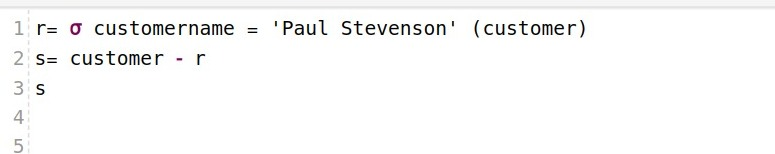
\includegraphics[width=5cm]{resources/pregunta2/3.1.1}
\end{center}

Así obtenemos el siguiente árbol de consulta
\begin{center}
    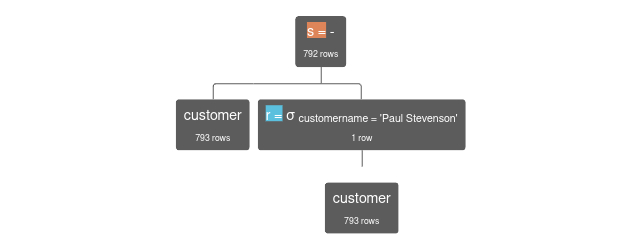
\includegraphics[width=7cm]{resources/pregunta2/3.1.2}
\end{center}
Y el resultado:
\begin{center}
    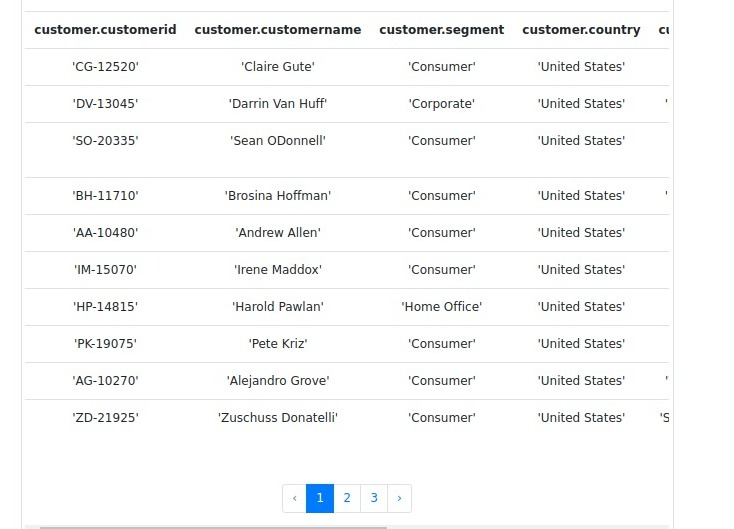
\includegraphics[width=9cm]{resources/pregunta2/3.1.3}
\end{center}

Si lo hacemos con sql obtenemos los mismos resultados
\begin{center}
    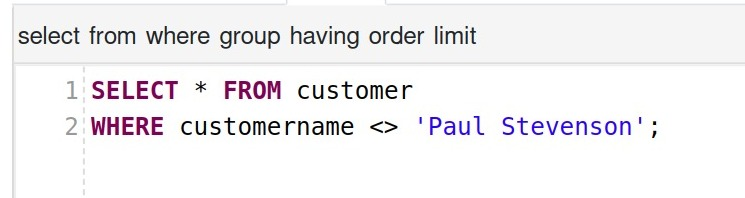
\includegraphics[width=5cm]{resources/pregunta2/3.1.4}
\end{center}
